\documentclass[11pt,a4paper]{article}

% --- Packages ---
\usepackage[utf8]{inputenc}
\usepackage[margin=1in]{geometry}
\usepackage{amsmath,amssymb}
\usepackage{graphicx}
\usepackage{booktabs}
\usepackage{listings}
\usepackage{xcolor}
\usepackage{fancyhdr}
\usepackage{microtype}
\usepackage{tikz}
\usetikzlibrary{arrows.meta, positioning, shapes.geometric, shapes.misc, calc}

% --- Hyperref Setup ---
\usepackage{hyperref}
\hypersetup{
    colorlinks=true,
    linkcolor=blue,
    citecolor=red,
    urlcolor=teal,
    pdftitle={WebRTC NAT Traversal and the NAT Problem},
    pdfauthor={MeetFlow Engineering Team}
}
\usepackage{cleveref}

% --- Custom Page Layout ---
\pagestyle{fancy}
\fancyhf{}
\setlength{\headheight}{14.5pt}
\rhead{\textbf{WebRTC Documentation}}
\lhead{NAT Traversal \& P2P Communication}
\rfoot{Page \thepage}
\lfoot{Confidential - For Internal Use Only}
\renewcommand{\headrulewidth}{0.4pt}
\renewcommand{\footrulewidth}{0.4pt}

% --- Code Block Style ---
\definecolor{codegray}{rgb}{0.96,0.96,0.96}
\definecolor{codeblue}{rgb}{0.1,0.2,0.6}
\definecolor{codegreen}{rgb}{0.1,0.5,0.1}

\lstset{
    backgroundcolor=\color{codegray},
    basicstyle=\small\ttfamily,
    breakatwhitespace=false,
    breaklines=true,
    captionpos=b,
    commentstyle=\color{codegreen},
    keywordstyle=\color{codeblue},
    numbers=left,
    numberstyle=\tiny\color{gray},
    numbersep=5pt,
    showspaces=false,
    showstringspaces=false,
    showtabs=false,
    tabsize=2,
    frame=single,
    rulecolor=\color{lightgray}
}

% --- Document Info ---
\title{
    \vspace{1.5in}
    \Huge \textbf{WebRTC NAT Traversal} \\
    \Large Deep-Dive: Why NAT Poses a Problem for Peer-to-Peer Networks \\
    \vspace{0.5in}
    \huge \textbf{Detailed Technical Report}
    \vspace{1.5in}
}
\author{
    \textbf{MeetFlow Engineering Team}
}
\date{\today}

\begin{document}

\maketitle
\thispagestyle{empty}
\newpage

\tableofcontents
\newpage

% =========================================================================
\section{Introduction}
% =========================================================================

The primary architectural goal of WebRTC (Web Real-Time Communication) is to establish a direct, \textbf{Peer-to-Peer (P2P)} connection between two web browsers. This design enables the exchange of audio, video, and arbitrary data channels with minimal latency, bypasses central server scaling limitations, and guarantees end-to-end encryption.

However, in the real-world Internet, establishing a direct connection between two arbitrary nodes is challenging. The main obstacle is \textbf{Network Address Translation (NAT)}. Designed initially as a temporary solution to mitigate IPv4 address exhaustion, NAT has become a ubiquitous standard in modern home routers, enterprise firewalls, and cellular networks. While NAT successfully connects private networks to the public Internet, it fundamentally breaks the end-to-end reachability model required for P2P protocols like WebRTC.

This document details why NAT complicates P2P communication, explains the underlying networking failures, and shows how protocols like STUN, ICE, and TURN work together to resolve these issues.

% =========================================================================
\section{Scenario 1: Peer-to-Peer Without NAT (The Ideal Case)}
% =========================================================================

To understand the problems introduced by NAT, consider an ideal network environment where every client device has a unique, globally routable \textbf{Public IP Address}. 

Suppose two clients wish to connect:
\begin{itemize}
    \item \textbf{Client 1:} Public IP address \texttt{49.32.100.8}
    \item \textbf{Client 2:} Public IP address \texttt{103.45.20.15}
\end{itemize}

Since both IP addresses are public, the global Internet routing system (routers, switches, and ISPs) knows exactly how to forward IP packets between these endpoints. Client 1 can construct a UDP packet with the destination set to \texttt{103.45.20.15} and send it. The packet is routed directly to Client 2. Similarly, Client 2 can respond directly to Client 1.

\begin{figure}[h!]
\centering
\resizebox{0.9\textwidth}{!}{%
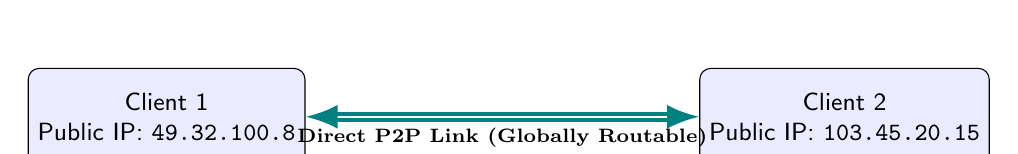
\begin{tikzpicture}[
    node distance=1.5cm and 2.5cm,
    client/.style={draw, fill=blue!8, rectangle, minimum height=3.5em, minimum width=10em, rounded corners, align=center, font=\small\sffamily},
    line/.style={draw, <->, >=Latex, double, color=teal, line width=1.5pt}
]
    \node[client] (c1) {Client 1\\Public IP: \texttt{49.32.100.8}};
    \node[client, right=5cm of c1] (c2) {Client 2\\Public IP: \texttt{103.45.20.15}};
    
    \draw[line] (c1) -- (c2) node[midway, below, font=\scriptsize\bfseries, color=black] {Direct P2P Link (Globally Routable)};
\end{tikzpicture}%
}
\caption{Scenario 1: Ideal Peer-to-Peer Connection without NAT}
\label{fig:ideal_no_nat}
\end{figure}

In this scenario, WebRTC session negotiation requires only the exchange of IP addresses and ports via a simple signaling server. Once the exchange completes, media flows directly between the clients without any issues.

\newpage

% =========================================================================
\section{Scenario 2: Peer-to-Peer with NAT (The Real-World Case)}
% =========================================================================

In reality, home and corporate networks utilize private subnets. Devices behind a router do not have unique public IP addresses. Instead, they are assigned \textbf{Private IP Addresses} that are only valid within their local network.

Consider a real-world configuration:
\begin{itemize}
    \item \textbf{User A (Local Client):}
    \begin{itemize}
        \item Laptop IP (Private): \texttt{192.168.1.10}
        \item Router A Public IP (WAN): \texttt{49.32.100.8}
    \end{itemize}
    \item \textbf{User B (Remote Client):}
    \begin{itemize}
        \item Laptop IP (Private): \texttt{192.168.0.5}
        \item Router B Public IP (WAN): \texttt{103.45.20.15}
    \end{itemize}
\end{itemize}

\begin{figure}[h!]
\centering
\resizebox{\textwidth}{!}{%
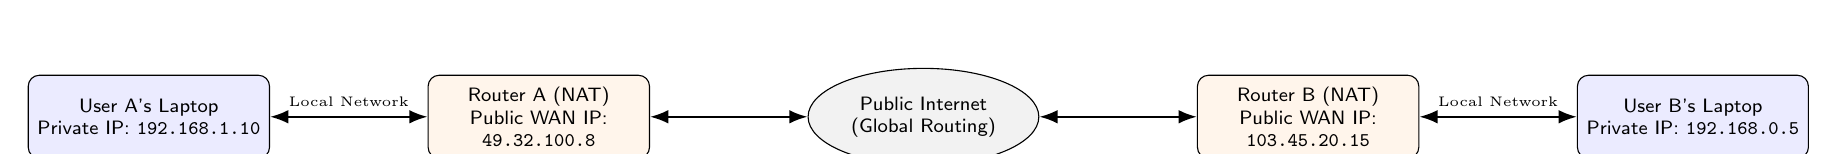
\begin{tikzpicture}[
    node distance=1.5cm and 2cm,
    client/.style={draw, fill=blue!8, rectangle, minimum height=3em, minimum width=8em, rounded corners, align=center, font=\scriptsize\sffamily},
    router/.style={draw, fill=orange!8, rectangle, minimum height=3em, minimum width=8em, rounded corners, align=center, font=\scriptsize\sffamily},
    internet/.style={draw, fill=gray!10, ellipse, minimum height=3.5em, minimum width=7em, align=center, font=\scriptsize\sffamily},
    line/.style={draw, -{Latex[scale=0.8]}, thick},
    biLine/.style={draw, <->, >=Latex, thick}
]

    % Nodes
    \node[client] (laptopA) {User A's Laptop\\Private IP: \texttt{192.168.1.10}};
    \node[router, right=2cm of laptopA] (routerA) {Router A (NAT)\\Public WAN IP:\\\texttt{49.32.100.8}};
    \node[internet, right=2cm of routerA] (internet) {Public Internet\\(Global Routing)};
    \node[router, right=2cm of internet] (routerB) {Router B (NAT)\\Public WAN IP:\\\texttt{103.45.20.15}};
    \node[client, right=2cm of routerB] (laptopB) {User B's Laptop\\Private IP: \texttt{192.168.0.5}};

    % Connections
    \draw[biLine] (laptopA) -- (routerA) node[midway, above, font=\tiny] {Local Network};
    \draw[biLine] (routerA) -- (internet);
    \draw[biLine] (internet) -- (routerB);
    \draw[biLine] (routerB) -- (laptopB) node[midway, above, font=\tiny] {Local Network};
    
\end{tikzpicture}%
}
\caption{Scenario 2: Real-World Network Architecture with NAT Interfaces}
\label{fig:real_world_nat}
\end{figure}

Under this structure, if Laptop A tries to communicate directly with Laptop B using standard P2P methods, it faces several major problems.

% =========================================================================
\section{The Three Core Problems of NAT in P2P}
% =========================================================================

\subsection{Problem 1: Non-Routable Private IP Addresses}
The IP addresses assigned to laptops inside local networks belong to reserved private address spaces:
\begin{itemize}
    \item \texttt{192.168.0.0} -- \texttt{192.168.255.255} (Class C)
    \item \texttt{10.0.0.0} -- \texttt{10.255.255.255} (Class A)
    \item \texttt{172.16.0.0} -- \texttt{172.31.255.255} (Class B)
\end{itemize}

According to RFC 1918, these addresses are strictly non-routable on the public Internet. Global Internet routers are configured to drop any packet containing a private destination IP address. 

If User B sends their local IP (\texttt{192.168.0.5}) in their WebRTC Session Description Protocol (SDP) offer, User A will attempt to send media packets to \texttt{192.168.0.5}. Since this is a private IP, User A's operating system or router will fail to route the packet to the WAN, or the packet will be dropped by the local ISP. Media transmission fails.

\subsection{Problem 2: NAT Port-Binding and Incoming Packet Filtering}
To bridge the gap between private and public IP networks, routers use a \textbf{NAT Mapping Table}. 

When Laptop A sends an outgoing request (e.g., fetching a webpage at \texttt{192.0.2.1:80}), the router intercepts the packet. It replaces the source private IP and port with its own public WAN IP and a dynamically selected port. It then adds a mapping entry to its NAT table:

\begin{table}[h!]
\centering
\begin{tabular}{ccccc}
\toprule
\textbf{Private Source IP} & \textbf{Private Port} & $\rightarrow$ & \textbf{Public Translated IP} & \textbf{Public Translated Port} \\
\midrule
\texttt{192.168.1.10} & \texttt{5000} & $\rightarrow$ & \texttt{49.32.100.8} & \texttt{62000} \\
\bottomrule
\end{tabular}
\caption{Example NAT Mapping Table Entry on Router A}
\label{tab:nat_table}
\end{table}

When the destination server sends a response back to \texttt{49.32.100.8:62000}, Router A checks its mapping table, sees that port \texttt{62000} corresponds to Laptop A (\texttt{192.168.1.10:5000}), modifies the destination header, and forwards the packet to the laptop.

\subsubsection{The Unsolicited Incoming Packet Problem}
Suppose Laptop A knows Laptop B's public IP address (\texttt{103.45.20.15}) and sends a packet directly to it on port \texttt{5000}.
When the packet reaches Router B:
\begin{enumerate}
    \item Router B receives a packet addressed to \texttt{103.45.20.15:5000}.
    \item Router B checks its active NAT Mapping Table.
    \item If Laptop B has not previously sent a packet \textit{outbound} to Laptop A's public IP and port from its local port \texttt{5000}, no mapping entry exists in Router B's table.
    \item Router B cannot determine which local device (\texttt{192.168.0.2}, \texttt{192.168.0.3}, or \texttt{192.168.0.5}) should receive the packet.
    \item For security, Router B drops the packet as unsolicited incoming traffic.
\end{enumerate}

\begin{figure}[h!]
\centering
\resizebox{0.9\textwidth}{!}{%
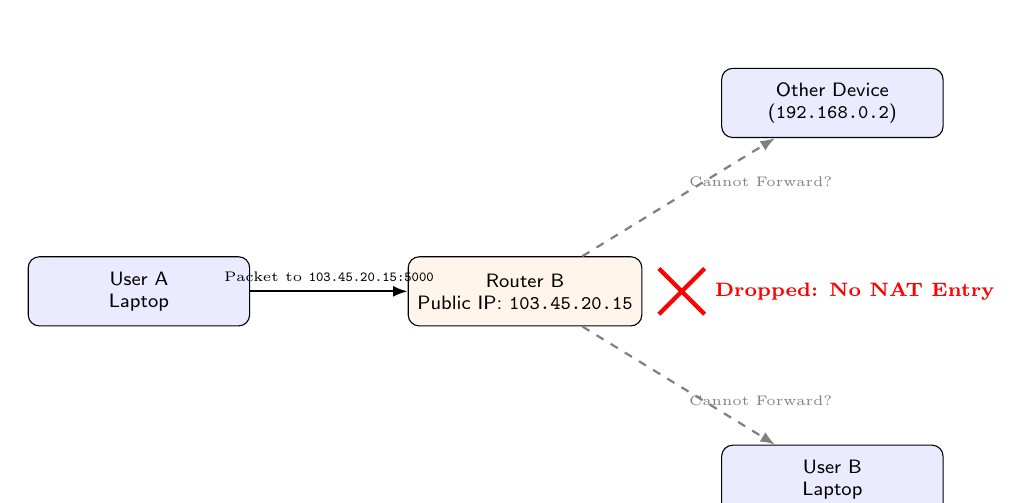
\begin{tikzpicture}[
    node distance=1.5cm and 2cm,
    client/.style={draw, fill=blue!8, rectangle, minimum height=2.5em, minimum width=8em, rounded corners, align=center, font=\scriptsize\sffamily},
    router/.style={draw, fill=orange!8, rectangle, minimum height=2.5em, minimum width=8em, rounded corners, align=center, font=\scriptsize\sffamily},
    line/.style={draw, -{Latex[scale=0.8]}, thick},
    cross/.style={draw, cross out, minimum size=15pt, line width=1.5pt, red}
]
    \node[client] (c1) {User A\\Laptop};
    \node[router, right=2cm of c1] (rB) {Router B\\Public IP: \texttt{103.45.20.15}};
    \node[client, below right=1.5cm and 1cm of rB] (c2) {User B\\Laptop};
    \node[client, above right=1.5cm and 1cm of rB] (c3) {Other Device\\(\texttt{192.168.0.2})};

    \draw[line] (c1) -- (rB) node[midway, above, font=\tiny] {Packet to \texttt{103.45.20.15:5000}};
    
    % Drop symbol at Router B
    \node[cross] at ($(rB.east) + (0.5,0)$) {};
    \node[red, right=0.8cm of rB, font=\scriptsize\bfseries] {Dropped: No NAT Entry};
    
    \draw[line, dashed, color=gray] (rB) -- (c2) node[midway, below right, font=\tiny] {Cannot Forward?};
    \draw[line, dashed, color=gray] (rB) -- (c3) node[midway, above right, font=\tiny] {Cannot Forward?};
\end{tikzpicture}%
}
\caption{The Incoming Packet Forwarding Problem}
\label{fig:incoming_drop}
\end{figure}

\subsection{Problem 3: Mutual Isolation (The Double-NAT Lockout)}
If both User A and User B are behind separate NAT routers, they face a mutual lockout:
\begin{itemize}
    \item User A cannot send a packet to User B's public IP because Router B has no mapping and will drop it.
    \item User B cannot send a packet to User A's public IP because Router A has no mapping and will drop it.
    \item Neither side can initiate the connection because the initial packet is dropped before a mapping table entry can be created on the remote router.
\end{itemize}
This scenario is known as the \textbf{NAT Traversal Problem}.

\newpage

% =========================================================================
\section{How WebRTC Resolves NAT: STUN, ICE, and TURN}
% =========================================================================

To overcome these networking challenges, WebRTC relies on a suite of standard protocols: \textbf{STUN}, \textbf{ICE}, and \textbf{TURN}.

\subsection{STUN (Session Traversal Utilities for NAT)}
A STUN server is a public, lightweight utility hosted on the public Internet. It helps clients answer the question: \textit{"What is my public IP address and port as seen by the outside world?"}

The discovery flow proceeds as follows:
\begin{enumerate}
    \item Laptop A sends a UDP binding request to a public STUN server (e.g., \texttt{stun.l.google.com:19302}).
    \item The packet passes through Router A. Router A translates the source address and creates an entry in its NAT table (e.g., mapping \texttt{192.168.1.10:5000} to \texttt{49.32.100.8:62000}).
    \item The STUN server receives the packet from source \texttt{49.32.100.8:62000}.
    \item The STUN server inspects the packet header, extracts the public IP and port, wraps them inside a STUN response payload, and sends it back.
    \item Laptop A receives the STUN response and learns its public reflexive address: \texttt{49.32.100.8:62000}.
\end{enumerate}

\begin{figure}[h!]
\centering
\resizebox{0.9\textwidth}{!}{%
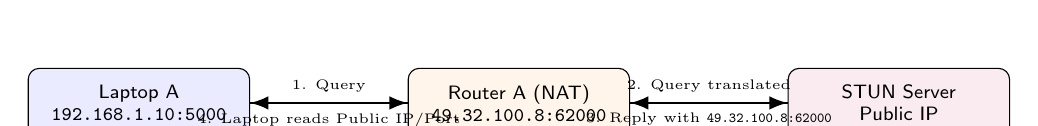
\begin{tikzpicture}[
    node distance=1.2cm and 2cm,
    client/.style={draw, fill=blue!8, rectangle, minimum height=2.5em, minimum width=8em, rounded corners, align=center, font=\scriptsize\sffamily},
    router/.style={draw, fill=orange!8, rectangle, minimum height=2.5em, minimum width=8em, rounded corners, align=center, font=\scriptsize\sffamily},
    server/.style={draw, fill=purple!8, rectangle, minimum height=2.5em, minimum width=8em, rounded corners, align=center, font=\scriptsize\sffamily},
    line/.style={draw, ->, >=Latex, thick},
    dashedline/.style={draw, dashed, ->, >=Latex, thick}
]
    \node[client] (laptop) {Laptop A\\\texttt{192.168.1.10:5000}};
    \node[router, right=2cm of laptop] (router) {Router A (NAT)\\\texttt{49.32.100.8:62000}};
    \node[server, right=2cm of router] (stun) {STUN Server\\Public IP};

    % Outgoing Query
    \draw[line] (laptop) -- (router) node[midway, above, font=\tiny] {1. Query};
    \draw[line] (router) -- (stun) node[midway, above, font=\tiny] {2. Query translated};

    % Incoming Response
    \draw[dashedline] (stun) -- (router) node[midway, below, font=\tiny] {3. Reply with \texttt{49.32.100.8:62000}};
    \draw[dashedline] (router) -- (laptop) node[midway, below, font=\tiny] {4. Laptop reads Public IP/Port};
\end{tikzpicture}%
}
\caption{STUN Public IP Discovery Mechanism}
\label{fig:stun_discovery}
\end{figure}

\subsection{ICE (Interactive Connectivity Establishment) Candidate Exchange}
Once both clients discover their public addresses (known as \textbf{Server Reflexive Candidates}) alongside their local LAN addresses (\textbf{Host Candidates}), they must exchange these network options.

Because they cannot communicate directly yet, they exchange these candidates using an intermediate \textbf{Signaling Server} (typically running WebSockets or Socket.IO):

\begin{figure}[h!]
\centering
\resizebox{0.8\textwidth}{!}{%
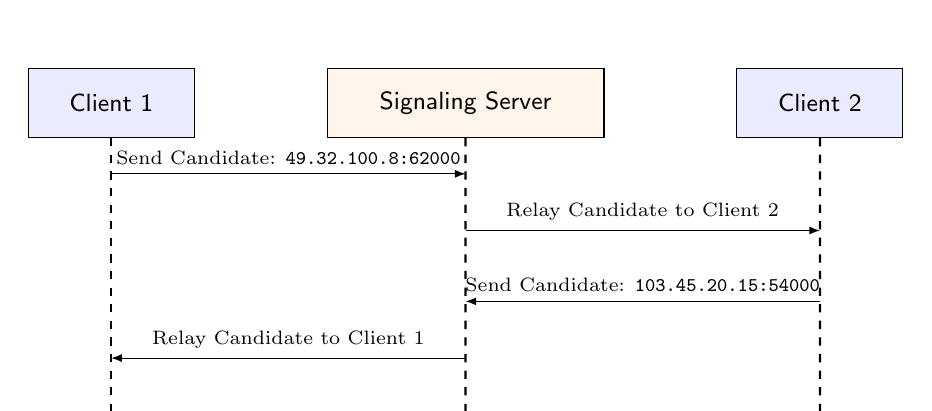
\begin{tikzpicture}[
    scale=0.9,
    every node/.style={font=\small\sffamily},
    actor/.style={draw, fill=blue!8, rectangle, minimum height=2.5em, minimum width=6em, align=center},
    server/.style={draw, fill=orange!8, rectangle, minimum height=2.5em, minimum width=10em, align=center}
]
    % Lifelines
    \node[actor] (A) at (0, 0) {Client 1};
    \node[server] (S) at (5, 0) {Signaling Server};
    \node[actor] (B) at (10, 0) {Client 2};
    
    \draw[dashed, thick] (A) -- (0, -4.5);
    \draw[dashed, thick] (S) -- (5, -4.5);
    \draw[dashed, thick] (B) -- (10, -4.5);

    % Exchange
    \draw[-{Latex[scale=0.8]}] (0, -1) -- (5, -1) node[midway, above, font=\scriptsize] {Send Candidate: \texttt{49.32.100.8:62000}};
    \draw[-{Latex[scale=0.8]}] (5, -1.8) -- (10, -1.8) node[midway, above, font=\scriptsize] {Relay Candidate to Client 2};
    
    \draw[-{Latex[scale=0.8]}] (10, -2.8) -- (5, -2.8) node[midway, above, font=\scriptsize] {Send Candidate: \texttt{103.45.20.15:54000}};
    \draw[-{Latex[scale=0.8]}] (5, -3.6) -- (0, -3.6) node[midway, above, font=\scriptsize] {Relay Candidate to Client 1};

\end{tikzpicture}%
}
\caption{ICE Candidate Exchange sequence via Signaling Server}
\label{fig:ice_exchange}
\end{figure}

\subsection{ICE Connectivity Checks (Hole Punching)}
Once candidate exchange completes, both browsers perform \textbf{Connectivity Checks} by sending STUN binding packets directly to each other's candidate addresses.

This process enables \textbf{Hole Punching}:
\begin{enumerate}
    \item Client 1 sends a packet to Client 2's public address (\texttt{103.45.20.15:54000}).
    \item Router 1 intercepts the packet and creates an outbound NAT mapping entry (allowing incoming packets from \texttt{103.45.20.15:54000} to reach Client 1).
    \item The packet arrives at Router 2. If Router 2 has not yet created a corresponding outbound mapping, it drops this first packet.
    \item Concurrently, Client 2 sends a packet to Client 1's public address (\texttt{49.32.100.8:62000}).
    \item Router 2 registers this outbound request, creating a mapping entry.
    \item When this packet reaches Router 1, Router 1 recognizes the source address (\texttt{103.45.20.15:54000}) because of the mapping created in Step 2. Router 1 forwards the packet to Client 1.
    \item Once Client 1 receives the packet, it sends a reply. Since Router 2 now has an active mapping entry for Client 1, the reply passes through.
    \item The direct peer-to-peer path is established.
\end{enumerate}

\newpage

% =========================================================================
\section{When P2P Fails: Symmetric NAT and TURN Servers}
% =========================================================================

Direct hole punching works with most home routers (which use Full Cone, Restricted Cone, or Port Restricted Cone NAT). However, it fails when one or both networks use a strict NAT type, such as \textbf{Symmetric NAT}, commonly found in corporate networks, enterprise firewalls, and 3G/4G/5G mobile carriers.

\subsection{Symmetric NAT Behavior}
Under Symmetric NAT, the router does not reuse the same public port mapping for different destination IPs. If Client 1 sends packets from port \texttt{5000} to two different destination IPs, the router creates two distinct public port mappings:
\begin{itemize}
    \item Outgoing to STUN Server $\rightarrow$ Mapped to \texttt{49.32.100.8:62000}
    \item Outgoing to Client 2 $\rightarrow$ Mapped to \texttt{49.32.100.8:63500}
\end{itemize}
Because the STUN server only observes port \texttt{62000}, Client 1 tells Client 2 to connect to port \texttt{62000}. However, when Client 2 attempts to send packets to \texttt{49.32.100.8:62000}, the symmetric router drops them because that mapping is restricted exclusively to traffic originating from the STUN server's IP address. Direct hole punching fails.

\subsection{TURN (Traversal Using Relays around NAT)}
When direct connection pathways fail, WebRTC falls back to a \textbf{TURN Server}. A TURN server acts as a media relay. Both clients establish connection legs to the TURN server, which forwards media packets between them.

While this approach guarantees that the call succeeds, it is no longer peer-to-peer:
\begin{itemize}
    \item \textbf{Latency:} Media packets must travel through the TURN server, increasing latency.
    \item \textbf{Cost:} The service provider must pay for the server bandwidth consumed by the relayed media.
    \item \textbf{Scale:} The TURN server must scale horizontally to handle high media throughput.
\end{itemize}

\begin{figure}[h!]
\centering
\resizebox{0.9\textwidth}{!}{%
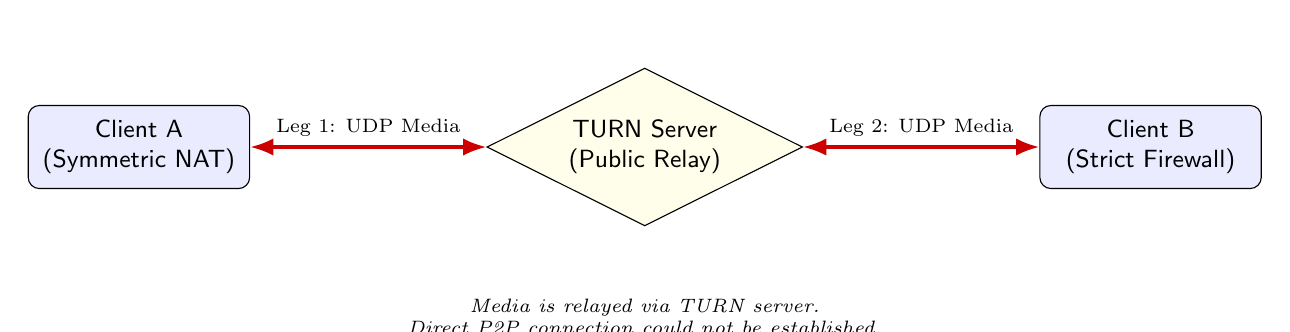
\begin{tikzpicture}[
    node distance=1.5cm and 2cm,
    client/.style={draw, fill=blue!8, rectangle, minimum height=3em, minimum width=8em, rounded corners, align=center, font=\small\sffamily},
    turn/.style={draw, fill=yellow!8, diamond, aspect=2.0, minimum width=8em, align=center, font=\small\sffamily},
    line/.style={draw, ->, >=Latex, thick, color=red!80!black, line width=1.2pt}
]
    \node[client] (c1) {Client A\\(Symmetric NAT)};
    \node[turn, right=3cm of c1] (turnServer) {TURN Server\\(Public Relay)};
    \node[client, right=3cm of turnServer] (c2) {Client B\\(Strict Firewall)};

    \draw[line, <->] (c1) -- (turnServer) node[midway, above, font=\scriptsize, color=black] {Leg 1: UDP Media};
    \draw[line, <->] (turnServer) -- (c2) node[midway, above, font=\scriptsize, color=black] {Leg 2: UDP Media};

    \node[below=0.8cm of turnServer, align=center, font=\scriptsize\itshape] {Media is relayed via TURN server. \\ Direct P2P connection could not be established.};
\end{tikzpicture}%
}
\caption{WebRTC Media Flow Relayed via a TURN Server}
\label{fig:turn_relay}
\end{figure}

% =========================================================================
\section{Summary: The WebRTC Connection Lifecycle}
% =========================================================================

The following checklist summarizes the sequence of events during a WebRTC connection attempt:

\begin{enumerate}
    \item \textbf{Candidate Gathering:} Both clients query local interfaces (Host Candidates) and STUN servers (Server Reflexive Candidates).
    \item **SDP Exchange:** Clients exchange these candidates along with media descriptors (codecs, encryption keys) through the Signaling Server.
    \item **Hole Punching:** Clients attempt direct UDP communication using the exchanged candidates.
    \item **Fallback to TURN:** If direct paths fail due to Symmetric NAT or firewalls, the connection transitions to a relayed path via a TURN server.
\end{enumerate}

This multi-tiered approach allows WebRTC to establish direct, low-latency P2P connections in over 85\% of standard consumer network configurations, falling back to TURN relays only when necessary.

\end{document}
